\documentclass[a4paper,12pt]{report}

\usepackage{cmap} % поиск в документе
\usepackage[T2A]{fontenc} % кодировка
\usepackage[utf8]{inputenc} % кодировка исходного текста
\usepackage[english, russian]{babel} % локализация и переносы

\usepackage{hyperref}

%%% Работа с картинками
\usepackage{graphicx}  % Для вставки рисунков
%\setlength\fboxsep{3pt} % Отступ рамки \fbox{} от рисунка
%\setlength\fboxrule{1pt} % Толщина линий рамки \fbox{}
%\usepackage{wrapfig} % Обтекание рисунков и таблиц текстом

\author{Колобов Кирилл, 201-321}
\date{}
\title{Аборты: геноцид или выбор?}

\begin{document}
\maketitle
\tableofcontents


\chapter{Введение}
Аборты -- частая причина разногласий между умудрённым опытом, годами старшим поколением с консервативными взгядами и идеологически прокачанными детьми -- леволиберальными проститутками.

Здесь разбираются основные положения споров, показывается аргументативная несостоятельность одной из сторон.

\chapter{За аборты}
    \section{Зигота -- не человек}
        Зигота не является человеком, это всего лишь кусок мяса.
    \section{Человек начинается с рождения}
        Зародыш становится человеком после рождения, ребёнок получает свидетельство о рождении.
    \section{Зигота -- часть тела матери}
        Зигота не может существовать вне тела матери, без потпитки оттуда $\Rightarrow$ зигота -- часть тела матери.
    \section{У зиготы нет разума}
        Зигота не разумна, она не может реагировать ни на какие раздражители извне.
    \section{Зигота -- не личность}
        У зиготы не мозга, она ещё не сформировалась, она не личность.
    \section{У матери есть выбор}
        Женщина хочет убить паразита, чтобы не кормить его и не мучаться.
    \section{Ты хочешь плодить нищету?}
        Если ребёнок родится, то он будет жить в нищите, он будет нежеланным. Ты этого хочешь?
    \section{Мать не хотела заводить ребёнка}
        Мать не хотела заводить ребёнка, она против этого, она ещё не готова.
    \section{Нет дня зачатия, есть день рождения}
        Никто не празднует день зачатия, все праздную день рождения.
    \section{По закону можно}
        Какие могут быть вопросы, если законом разрешено?
    \section{А если это было изнасилование?}
        А если это было изнасилование, то тоже нельзя сделать аборт? Женщине рожать ребёнка от насильника?

\chapter{Против абортов}
	\section{Зигота -- человек}
    %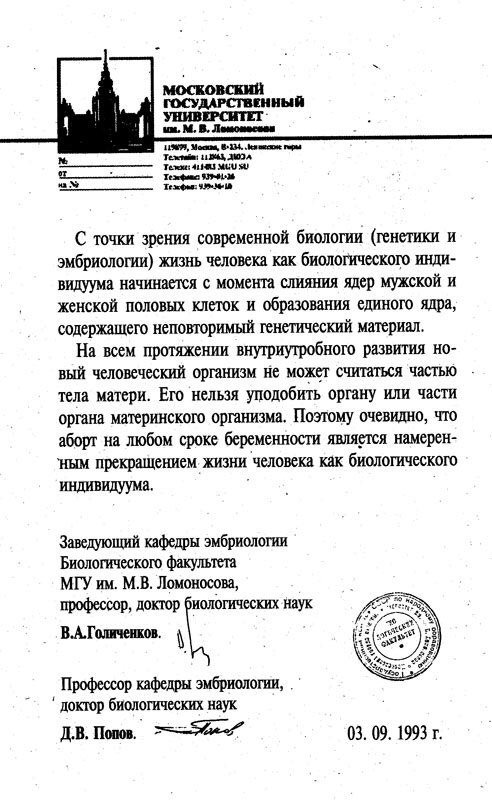
\includegraphics[scale=0.5]{evidence.}\label{evidence}
	\section{Человек начинается с зачатия}
        Зигота -- это первая стадия развития человеческого организма, небиологическое делеение -- арбитрарное, не иммет верифицируемых критериев.
	\section{Зигота -- новый организм}
        См рис. %\rel{evidence}
    \section{У тебя тоже}
    \section{Ты тоже}
	\section{Можно убить новорожденного?}
	\section{А чем думала мать?}
	\section{А чем думала мать?}
	\section{Контингентно культуре}
	\section{}
	\section{}
    \section{}

\chapter{Выводы}
Проблемы абортов, их распространённость и необходимость, у многих наслуху неспроста: современному среднечеловеку чуждо чувство отвественности, он не готов ни думать о своих действиях заранее, ни принимать последствия совершённых ошибок -- незащищённого секса, в данном случае.

Решение этой проблемы пустоголовые создания видят в массовом геноциде определённой группы людей, самых незащищённых из нас --  нерождённых. 

При этом, к сожалению, процесс мышления (как и любовь до гроба, крепкая семья) из моды выходит, вследствие этого простая альтернатива гуляет перед лицом у \textit{homo consumer} незамеченной. 

Впрочем, предлагаемая альтернатива решит также проблему неизлечимых (а впрочем, излечимых тоже) венирических болезней: ВИЧ, его запущенная форма -- СПИД, сифилис, хламидиоз, трихомониаз et cetera.

И альтернатива эта (барабанная дробь!) -- защищённый секс.
\end{document}
